\documentclass[11pt,a4paper]{article}
\usepackage[utf8]{inputenc}
\usepackage[T1]{fontenc}
\usepackage{lmodern}
\usepackage[spanish,es-noquoting]{babel}
\usepackage{amsmath,amssymb,bm}
\usepackage{graphicx}
\usepackage{booktabs}
\usepackage[margin=2.1cm]{geometry}
\usepackage{xcolor}
\usepackage[font=small,labelfont=bf]{caption}
\usepackage{float}
\usepackage[section]{placeins}
\usepackage{microtype}
\usepackage[colorlinks=true,linkcolor=blue!50!black,urlcolor=blue!50!black]{hyperref}
\graphicspath{{fig/}}
\setlength{\parskip}{4pt}
\setlength{\parindent}{0pt}
\newcommand{\code}[1]{\texttt{#1}}
\newcommand{\dd}{\,\mathrm{d}}
\newcommand{\atan}{\operatorname{atan2}}

\title{\vspace{-1.2cm}Segway con patas: cinemática y dinámica del modelo\\[4pt]
\large Notación, deducción y valores, para revisión del grupo}
\author{Robótica II, UNCUYO. Generado con Claude Code sobre el repositorio del grupo}
\date{3 de septiembre de 2026}

\begin{document}
\maketitle
\vspace{-0.8cm}

\paragraph{Alcance.} Este documento explica sólo dos cosas: cómo se calcula la cinemática de la pata
(directa e inversa) y cómo se dedujo la dinámica del robot que usa la planta de
\code{simulacion/planta\_v1/}. Cada símbolo está definido en la figura~\ref{fig:cin} o en la
figura~\ref{fig:din} y en el cuadro~\ref{tab:simb}. El control, los sensores y los resultados de
simulación quedan para otro informe. Las cotas y masas son las del CAD \code{primera\_iteracion}
(medidas sobre el STEP; ver \code{base\_conocimiento/dimensiones\_cad\_primera\_iteracion.md}).

\section{Notación y convenciones}

\begin{figure}[H]
  \centering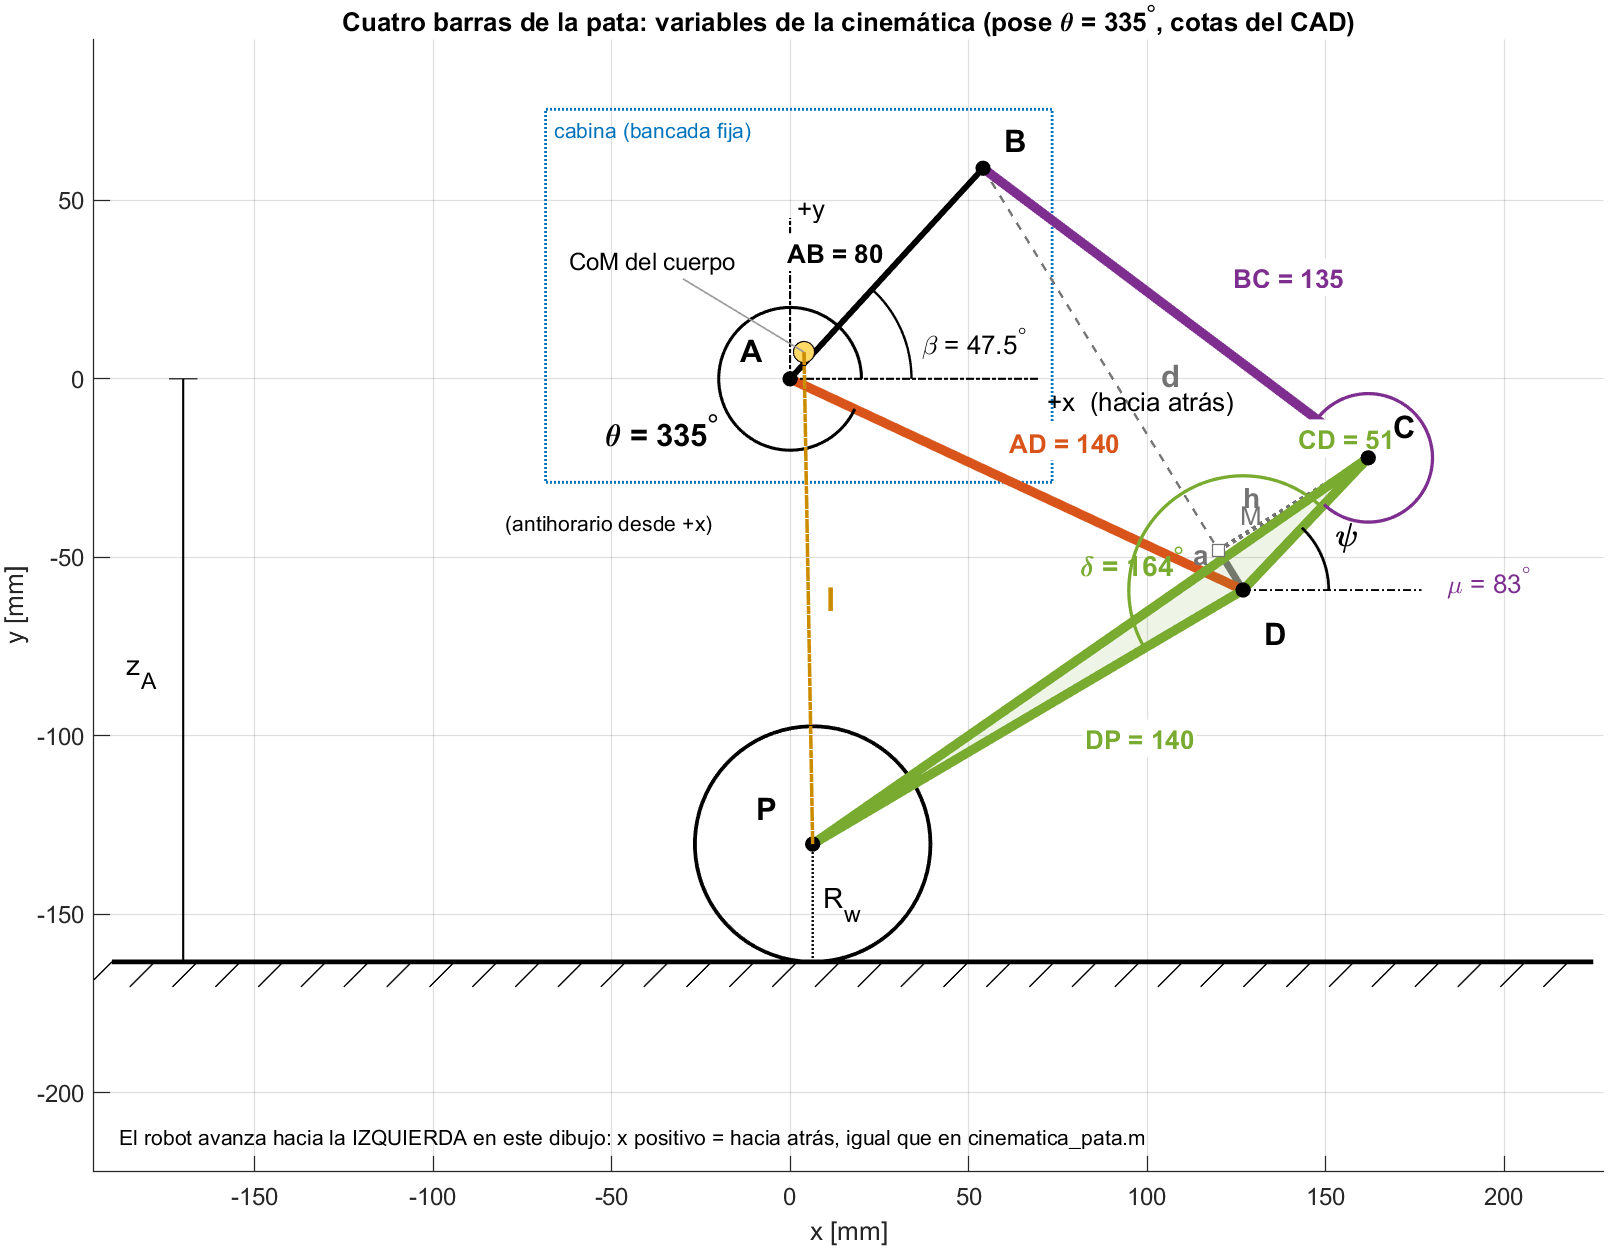
\includegraphics[width=0.98\textwidth]{fig_cinematica_anotada}
  \caption{Variables de la cinemática, dibujadas sobre la geometría real del CAD en la pose
  $\theta = 335^\circ $. Marco cinemático: origen en $A$, $x$ positivo \emph{hacia atrás}, $y$ hacia
  arriba; el robot avanza hacia la izquierda. Los ángulos se miden en sentido antihorario.}
  \label{fig:cin}
\end{figure}

Hay dos marcos y conviene tenerlos separados desde el principio:

\begin{itemize}\itemsep2pt
  \item \textbf{Marco cinemático} (fig.~\ref{fig:cin}, el de \code{cinematica\_pata.m} del grupo):
  origen en el eje del servo $A$, $x$ positivo hacia atrás, $y$ hacia arriba. Se eligió así porque
  la pata se pliega hacia atrás y todos los puntos $C$, $D$ quedan con $x > 0$.
  \item \textbf{Marco dinámico} (fig.~\ref{fig:din}): $x$ positivo \emph{hacia adelante} a lo largo del
  piso, que es la convención normal de un péndulo invertido. El pasaje entre marcos es un cambio de
  signo en $x$; las alturas ($y$, $z_A$, $l$) son las mismas.
\end{itemize}

\begin{table}[H]
  \centering\small
  \begin{tabular}{llp{9.2cm}}
    \toprule
    Símbolo & Valor CAD & Significado \\
    \midrule
    $A$, $B$ & $A=(0,0)$; $B = AB(\cos\beta,\sin\beta)$ & pivotes fijos en la cabina: $A$ eje del servo, $B$ pivote del balancín \\
    $AB$, $\beta$ & 80\,mm, 47{,}5° & bancada y su orientación respecto de $+x$ \\
    $AD$ & 140\,mm & manivela, la mueve el servo \\
    $BC$ & 135\,mm & balancín \\
    $CD$, $DP$, $\delta$ & 51\,mm, 140\,mm, 164° & acoplador: es \emph{una} pieza rígida $CDP$; $\delta$ es el ángulo de la dirección $D\!\to\!C$ a la dirección $D\!\to\!P$ \\
    $\theta$ & 320° a 350° & ángulo de la manivela $A\!\to\!D$ desde $+x$, antihorario. 320° = pata estirada (robot de pie), 350° = plegada \\
    $\psi$ & sale de la cinemática & ángulo de la dirección $D\!\to\!C$ desde $+x$ \\
    $\mu$ & 60° a 90° & ángulo de transmisión en $C$, entre $C\!\to\!D$ y $C\!\to\!B$ \\
    $\rho$ & $+1$ & rama de armado (de qué lado de la recta $BD$ queda $C$) \\
    $d, a, h, M$ & construcción & $d = |B-D|$; $M$ es el pie de la perpendicular desde $C$ a $BD$; $a = |D-M|$, $h = |C-M|$ \\
    $P$, $R_w$ & 33\,mm & eje de rueda y radio de rueda \\
    $z_A$ & 108 a 212\,mm & altura de $A$ sobre el piso: $z_A = R_w - P_y$ \\
    $\mathrm{CoM}$ & (3{,}9 atrás, 7{,}5 arriba) mm & centro de masa del cuerpo suspendido, respecto de $A$ \\
    $l$ & 83 a 186\,mm & distancia del eje de rueda al CoM del cuerpo: el largo del péndulo \\
    $G$ & 0{,}20\,m/rad & $|\dd l/\dd\theta|$, ganancia del mecanismo \\
    \midrule
    $x$, $\phi$ & & posición del eje a lo largo del piso; ángulo de la recta eje$\to$CoM desde la normal al piso (+ adelante) \\
    $\alpha$ & & pendiente del piso (+ subida hacia adelante); la IMU mide $\phi+\alpha$ \\
    $m_b$, $J_b$ & 0{,}78\,kg, $2{,}8\cdot10^{-3}$\,kg\,m$^2$ & masa e inercia (respecto de su CoM) del cuerpo suspendido \\
    $m_w$, $J_w$ & 0{,}25\,kg, $1{,}6\cdot10^{-5}$\,kg\,m$^2$ & masa en el eje (2 ruedas + 2 motores) e inercia de una rueda \\
    $\theta_w$, $\omega_w$ & & giro y velocidad de cada rueda \\
    $\theta_m$, $\omega_m$, $i$ & & giro, velocidad y corriente del rotor de cada motor \\
    $n_g$, $J_r$ & 100 (CAD) ó 21{,}3; $6\cdot10^{-7}$\,kg\,m$^2$ & relación del reductor e inercia del rotor \\
    $\tau_g$, $f$, $N$ & & par que el reductor aplica a la rueda; fuerza de piso tangencial; normal por rueda \\
    $\tau_s$, $n_s$, $F_l$ & $n_s = 2$ & par de cada servo, cantidad de servos, fuerza equivalente a lo largo de la pata \\
    $F_x$, $M_p$, $F_{esc}$ & & perturbaciones: fuerza en el CoM, momento de cabeceo, golpe horizontal en el eje \\
    \bottomrule
  \end{tabular}
  \caption{Símbolos. Valores del CAD tal como está (variante \code{cad}).}
  \label{tab:simb}
\end{table}

\section{Cinemática directa: de $\theta$ a $D$, $C$ y $P$}

\subsection{Construcción}

Se conoce $\theta$ y se buscan las posiciones de los tres puntos móviles. Con la notación de la
figura~\ref{fig:cin}:

\begin{enumerate}\itemsep3pt
  \item \textbf{Manivela.} $D$ gira alrededor de $A$:
  \begin{equation}
    D = A + AD\,(\cos\theta,\ \sin\theta).
    \label{eq:D}
  \end{equation}
  \item \textbf{Acoplador por intersección de circunferencias.} $C$ está a distancia $BC$ de $B$ y a
  distancia $CD$ de $D$. Sea $\bm v = B - D$ y $d = |\bm v|$. El pie de la perpendicular $M$ queda a
  distancia $a$ de $D$ sobre $DB$, y $C$ a distancia $h$ de $M$ en dirección perpendicular:
  \begin{equation}
    a = \frac{CD^2 - BC^2 + d^2}{2d}, \qquad h = \sqrt{CD^2 - a^2}, \qquad
    M = D + a\,\frac{\bm v}{d}, \qquad C = M + \rho\, h\,\frac{(v_y,\,-v_x)}{d}.
    \label{eq:C}
  \end{equation}
  La fórmula de $a$ sale de restar las dos ecuaciones de circunferencia, $|C-D|^2 = CD^2$ y
  $|C-B|^2 = BC^2$, con $|C-M|$ común: $a^2 + h^2 = CD^2$ y $(d-a)^2 + h^2 = BC^2$. El signo $\rho$
  elige una de las dos soluciones; $\rho = +1$ es la rama en la que está armado el CAD ($C$ del lado
  de $x$ mayor). El mecanismo cierra sólo si $|BC - CD| < d < BC + CD$.
  \item \textbf{Punto de rueda.} $P$ es solidario al acoplador: se gira $\delta$ desde la dirección
  $D\!\to\!C$ y se avanza $DP$:
  \begin{equation}
    \psi = \atan(C_y - D_y,\ C_x - D_x), \qquad P = D + DP\,\big(\cos(\psi+\delta),\ \sin(\psi+\delta)\big).
    \label{eq:P}
  \end{equation}
  Con $\delta = 164^\circ $, $P$ queda casi en la prolongación de $C\!\to\!D$ (el plano acota el
  suplementario, 16°, entre $DC$ y la prolongación de $PD$: no cargar 16 donde va 164).
  \item \textbf{Ángulo de transmisión.} Mide qué tan bien empuja el acoplador al balancín:
  \begin{equation}
    \cos\mu' = \frac{(D-C)\cdot(B-C)}{|D-C|\,|B-C|}, \qquad \mu = \min(\mu',\ \pi - \mu').
    \label{eq:mu}
  \end{equation}
  Cerca de 0° ó 180° el mecanismo se traba; en el CAD $\mu$ va de 60° a 90° en todo el recorrido.
\end{enumerate}

\subsection{Equivalencia con la deducción a mano del grupo}

En \code{modelado/cinematica/geometrico\_1.jpeg} y \code{\_2.jpeg} se hace la misma construcción
pero desde $B$: $\cos\beta_{BD} = (BC^2 + d^2 - CD^2)/(2\,BC\,d)$ por teorema del coseno y luego
$\theta_{BC} = \alpha_{BD} \pm \beta_{BD}$. Es la misma solución escrita desde el otro extremo de
$BD$: $BC\cos\beta_{BD} = d - a$. Las dos diferencias son de marco, no de método: allí $B$ se pone
sobre el eje $x$ ($B = (L, 0)$) y las barras se escriben como múltiplos de $L$; aquí $B$ queda en
su posición real del CAD, $B = 80\,(\cos 47{,}5^\circ ,\ \sin 47{,}5^\circ )$\,mm, y las barras van en mm para
que las coordenadas coincidan con el ensamble.

\subsection{Del eje de rueda a las alturas y al largo del péndulo}

El piso está a $R_w$ por debajo de $P$. Por lo tanto la altura de $A$ sobre el piso, la altura del
tope de la tapa (74{,}5\,mm sobre $A$ en el CAD) y el largo del péndulo son
\begin{equation}
  z_A = R_w - P_y, \qquad h_{tapa} = z_A + 0{,}0745, \qquad l = -P_y + y_{\mathrm{CoM}} .
  \label{eq:l}
\end{equation}
$l$ es la única salida de la cinemática que usa la dinámica. El desvío horizontal de $P$ respecto de
la vertical de $A$ (unos mm) no entra en $l$: en la dinámica $\phi$ es el ángulo de la recta
$P\!\to\!\mathrm{CoM}$, así que ese desvío se absorbe como una inclinación pequeña de la cabina en
equilibrio (hasta 4° en el CAD, 0{,}3° con la bancada corregida). Es una hipótesis a tener presente.

\subsection{Qué da con las cotas del CAD}

\begin{figure}[H]
  \centering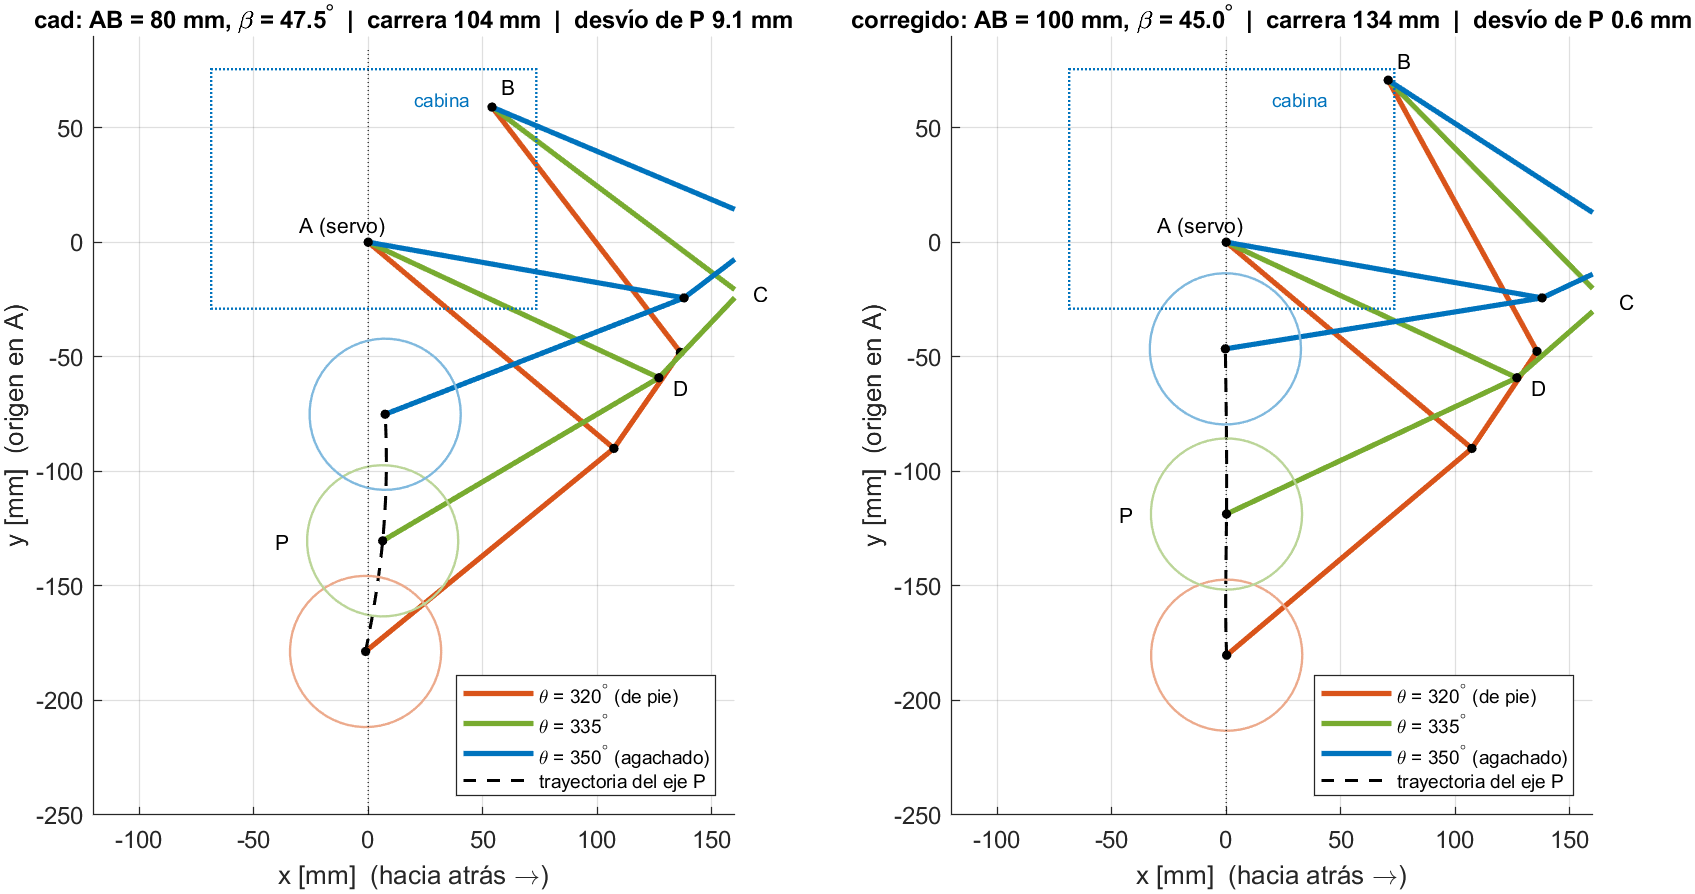
\includegraphics[width=\textwidth]{fig_mecanismo}
  \caption{Tres poses y trayectoria de $P$, en el marco cinemático. Izquierda: CAD tal como está.
  Derecha: bancada llevada a 100\,mm a 45°, que es la escala para la que se diseñaron las barras.}
  \label{fig:mec}
\end{figure}

\begin{table}[H]
  \centering\small
  \begin{tabular}{lrr}
    \toprule
     & CAD (AB = 80\,mm, $\beta$ = 47{,}5°) & corregido (AB = 100\,mm, $\beta$ = 45°) \\
    \midrule
    Carrera de $P$ entre 320° y 350° & 103{,}5\,mm & 133{,}7\,mm \\
    Desvío horizontal de $P$ & 9{,}1\,mm (8{,}7\,\%) & 0{,}6\,mm (0{,}4\,\%) \\
    $z_A$ de pie / agachado & 212 / 108\,mm & 246 / 108\,mm \\
    Tope de la tapa de pie / agachado & 286 / 182\,mm & 320 / 182\,mm \\
    $\mu$ mínimo & 60° & 58° \\
    Rango de $l$ & 83 a 186\,mm & 54 a 188\,mm \\
    \bottomrule
  \end{tabular}
  \caption{Cinemática directa evaluada en el recorrido del servo.}
\end{table}

Las barras del CAD son la familia \code{grupo} de \code{params\_robot.m} ($k_{AD} = 1{,}4$,
$k_{BC} = 1{,}35$, $k_{CD} = 0{,}51$, $k_{DP} = 1{,}4$) con escala $s = 100$\,mm, pero los pivotes de
\code{cabeza\_v31} están a 80\,mm. Como el cuatro barras no es invariante a escalar sólo la bancada,
la recta se degrada 15 veces. O se mueve $B$ en la cabina, o se reimprimen las barras a escala 80
(112, 108, 40{,}8, 112\,mm).

\section{Cinemática inversa: de $l$ (o de la altura) a $\theta$}

\subsection{Por qué se resuelve por tabla}

$\theta(l)$ no tiene expresión cerrada: $P$ depende de $\theta$ a través de la raíz de
\eqref{eq:C} y del giro \eqref{eq:P}. Lo que sí se cumple en el recorrido útil es que $l(\theta)$
es monótona (decrece cuando $\theta$ crece: plegar la pata acorta el péndulo), así que la inversa
es única. \code{parametros\_v1} evalúa \eqref{eq:D}--\eqref{eq:l} en 121 valores de $\theta$ y guarda
21 nodos equiespaciados en $l$ con $\theta(l)$ y $\dd\theta/\dd l$ (fig.~\ref{fig:mapa});
\code{interp\_lin} interpola linealmente con extrapolación fuera del rango. El error de interpolación
es menor que 0{,}1\,mm. Como cualquier altura de interés se convierte en $l$ con \eqref{eq:l}, la
misma tabla resuelve ``qué $\theta$ hace falta para tal altura''.

\begin{figure}[H]
  \centering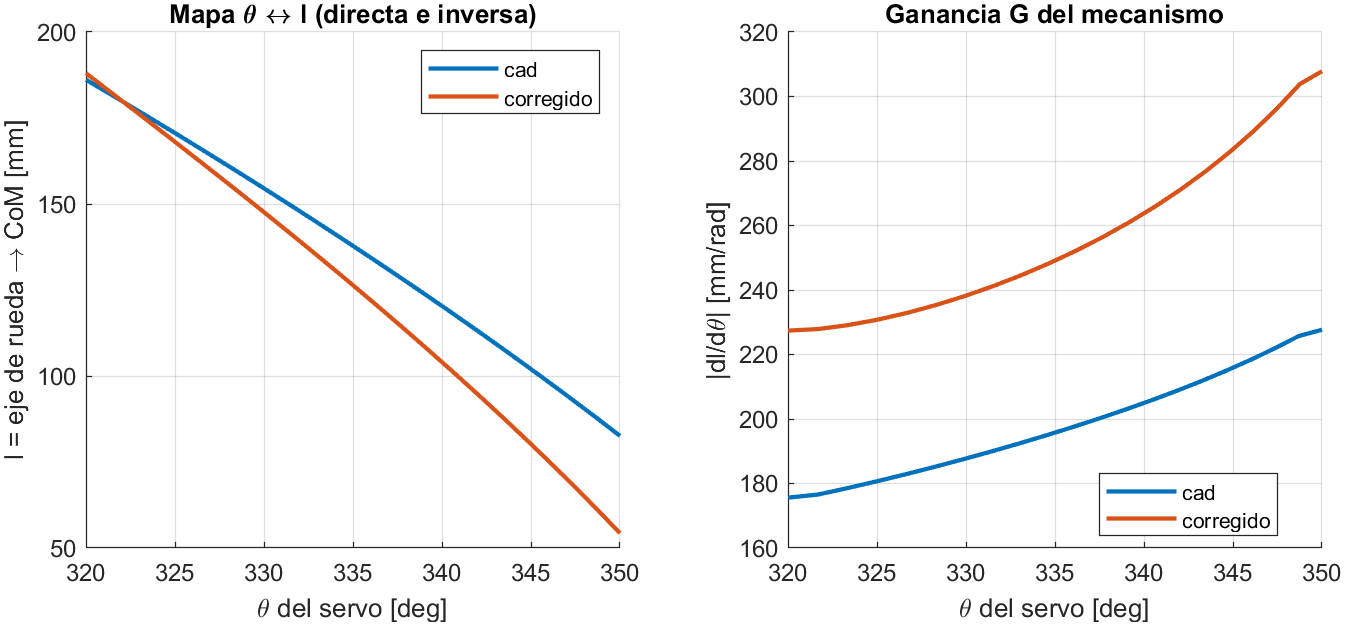
\includegraphics[width=0.95\textwidth]{fig_mapa_theta_l}
  \caption{Izquierda: $l(\theta)$, que se lee en cualquier sentido. Derecha: ganancia
  $G = |\dd l/\dd\theta|$.}
  \label{fig:mapa}
\end{figure}

\subsection{Velocidades y fuerzas: la ganancia $G$}

Derivando la tabla, $\dot l = (\dd l/\dd\theta)\,\dot\theta$. Por trabajo virtual, un par $\tau_s$ en
el hombro equivale a una fuerza $F$ a lo largo del péndulo:
\begin{equation}
  \tau_s\,\delta\theta = F\,\delta l \quad\Rightarrow\quad F_l = n_s\,\tau_s\,\frac{\dd\theta}{\dd l},
  \qquad \frac{\dd\theta}{\dd l} < 0 \text{ en esta geometría}.
  \label{eq:tv}
\end{equation}
El signo importa: $F_l > 0$ estira la pata, y para eso el servo tiene que \emph{bajar} $\theta$.
En módulo, $G = |\dd l/\dd\theta| \approx 0{,}2$\,m/rad significa que sostener el peso del cuerpo
($m_b g = 7{,}7$\,N) cuesta $m_b g\,G/n_s = 0{,}76$\,N\,m por servo; el DS3225MG da 2{,}4. Esta es la
relación que \code{params\_robot.m} llamaba ``dz/dtheta'' y que allí valía 204\,mm/rad a escala 80.

\section{Dinámica}

\subsection{Hipótesis}

\begin{enumerate}\itemsep2pt
  \item Movimiento en el plano sagital. Las dos patas están sincronizadas (mismo $\theta$) y los
  dos motores suman su par; no hay guiñada.
  \item El cuerpo suspendido (cabina, tapa, servos, batería, electrónica y las barras) es un rígido
  de masa $m_b$ e inercia $J_b$ con su CoM a distancia $l$ del eje de rueda. Las barras cambian de
  posición con $\theta$; su aporte al CoM y a $J_b$ se promedia sobre el recorrido. El cambio de $l$
  entra en la cinética como un grado de libertad prismático.
  \item Ruedas y motores ($m_w$) están en el eje; su altura sobre el piso es constante ($R_w$).
  \item La rueda \emph{no} rueda por definición: su giro es un estado propio y la fuerza de piso
  sale de un modelo de fricción, para poder representar deslizamiento.
  \item El piso es un plano de pendiente $\alpha$; la gravedad se rota, no el robot.
  \item El servo se modela como fuente de par con lazo interno; entra al cuerpo por \eqref{eq:tv}.
  La inercia propia del cuatro barras alrededor del hombro se desprecia.
\end{enumerate}

\begin{figure}[H]
  \centering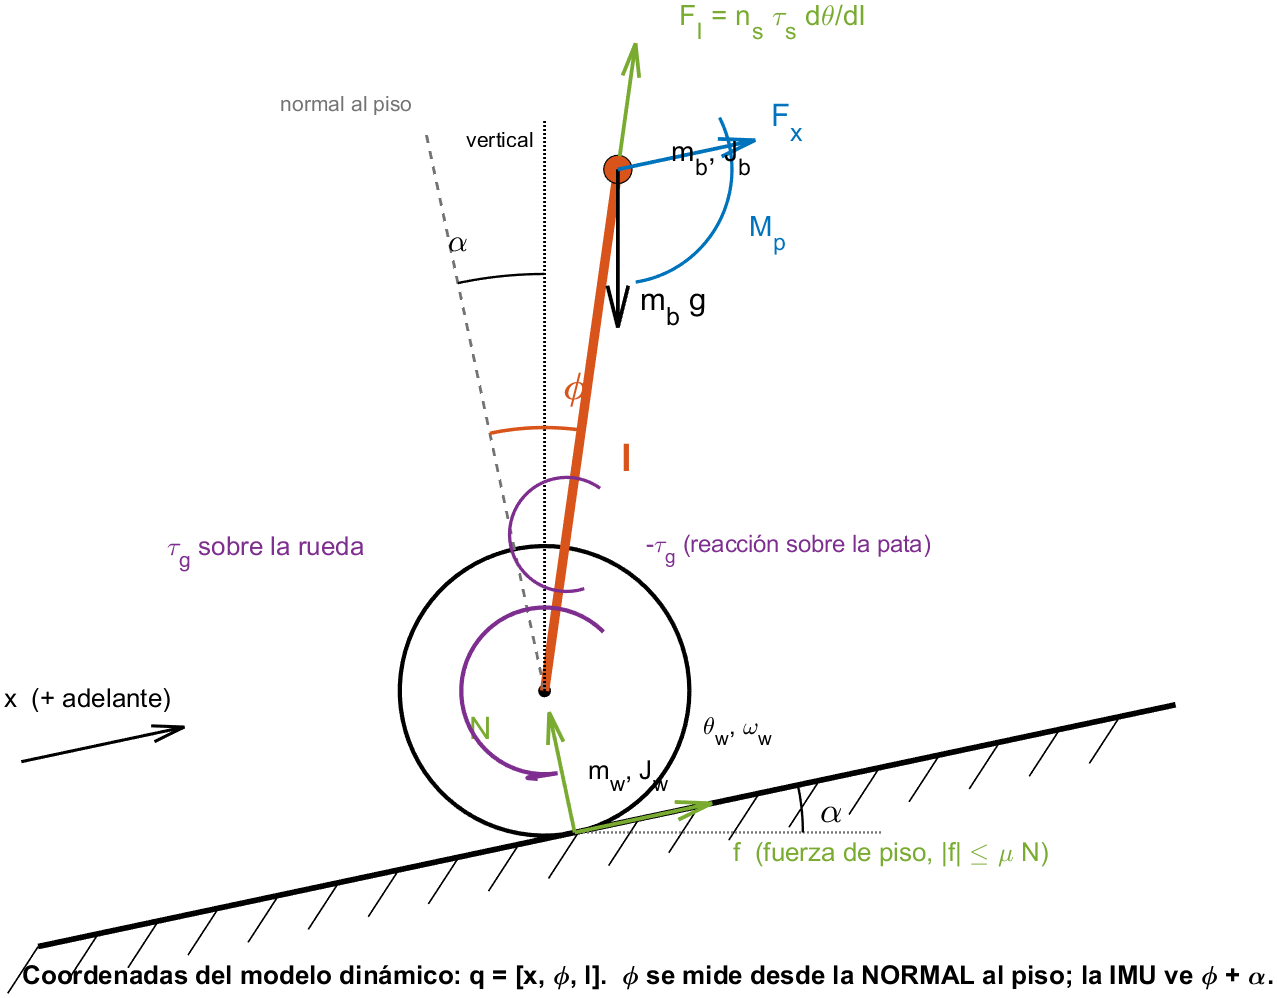
\includegraphics[width=0.8\textwidth]{fig_dinamica}
  \caption{Coordenadas generalizadas $q = [x,\phi,l]$ y todas las fuerzas y pares que entran en las
  ecuaciones, sobre un piso con pendiente $\alpha$. $\phi$ se mide desde la normal al piso, hacia
  adelante.}
  \label{fig:din}
\end{figure}

\subsection{Ecuaciones del cuerpo por Lagrange}

En el marco del piso (eje $x$ a lo largo del piso, $y$ normal), las posiciones del eje y del CoM son
\begin{equation}
  \bm r_w = (x,\ 0), \qquad \bm r_b = (x + l\sin\phi,\ l\cos\phi).
\end{equation}
Derivando, $\dot{\bm r}_b = (\dot x + \dot l\sin\phi + l\dot\phi\cos\phi,\ \dot l\cos\phi - l\dot\phi\sin\phi)$,
y la energía cinética y el potencial (gravedad rotada $\bm g = g(-\sin\alpha, -\cos\alpha)$) son
\begin{equation}
  T = \tfrac12 m_w\dot x^2 + \tfrac12 m_b\,|\dot{\bm r}_b|^2 + \tfrac12 J_b\dot\phi^2, \qquad
  V = -m_b\,\bm g\cdot\bm r_b - m_w\,\bm g\cdot\bm r_w .
\end{equation}
Las ecuaciones de Lagrange $\frac{\dd}{\dd t}\frac{\partial T}{\partial\dot q} - \frac{\partial T}{\partial q} + \frac{\partial V}{\partial q} = Q$
se escriben en la forma estándar
\begin{equation}
  M(q)\,\ddot q + C(q,\dot q) + G_v(q) = Q,
  \label{eq:lag}
\end{equation}
con $M = \partial^2 T/\partial\dot q^2$, $C$ los términos de Coriolis y centrífugos (símbolos de
Christoffel, $C_i = \sum_{j,k}\tfrac12(\partial_k M_{ij} + \partial_j M_{ik} - \partial_i M_{jk})\dot q_j\dot q_k$)
y $G_v = \partial V/\partial q$. La deducción se hizo con el Symbolic Math Toolbox
(\code{derivar\_dinamica\_v1.m}) y el resultado generado (\code{dinamica\_v1\_gen.m}) es
\begin{equation}
  M = \begin{bmatrix} m_b + m_w & m_b l\cos\phi & m_b\sin\phi \\[2pt] m_b l\cos\phi & J_b + m_b l^2 & 0 \\[2pt] m_b\sin\phi & 0 & m_b \end{bmatrix},\qquad
  C = \begin{bmatrix} m_b\dot\phi\,(2\dot l\cos\phi - l\dot\phi\sin\phi) \\[2pt] 2 m_b\, l\,\dot l\,\dot\phi \\[2pt] -m_b\, l\,\dot\phi^2 \end{bmatrix},
\end{equation}
\begin{equation}
  G_v = \begin{bmatrix} (m_b+m_w)\,g\sin\alpha \\[2pt] m_b\,g\,l\,\sin(\alpha-\phi) \\[2pt] m_b\,g\cos(\alpha-\phi) \end{bmatrix}.
\end{equation}
Lectura de $G_v$: en piso horizontal la segunda fila es $-m_b g l\sin\phi$, el par de vuelco del
péndulo invertido, y la tercera es $m_b g\cos\phi$, el peso que la pata tiene que sostener; con
pendiente aparece además la componente $g\sin\alpha$ del peso total a lo largo del piso. Con
$\alpha = 0$, $M$, $C$ y $G_v$ coinciden término a término con \code{dinamica\_sl.m} del grupo
(salvo que allí $M_{11}$ incluye $J_w/R_w^2$ porque la rueda rueda sin deslizar).

\subsection{Fuerzas generalizadas}

Cada fuerza real se proyecta sobre las coordenadas por trabajo virtual ($Q_i = \bm F\cdot\partial\bm r/\partial q_i$):
\begin{equation}
  Q = \begin{bmatrix}
      f_L + f_R + F_x + F_{esc} \\[3pt]
      -(\tau_{gL} + \tau_{gR}) + M_p + F_x\, l\cos\phi - b_\phi\,\dot\phi \\[3pt]
      F_l + F_x\sin\phi - b_l\,\dot l + f_{tope}
      \end{bmatrix}.
  \label{eq:Q}
\end{equation}
\begin{itemize}\itemsep2pt
  \item \textbf{Fuerza de piso} $f_L + f_R$: actúa en el contacto, pero como el eje está a altura fija
  y las ruedas son estados aparte, sobre el cuerpo entra sólo como fuerza en $x$.
  \item \textbf{Reacción del motor} $-\tau_g$: el estator y el reductor van fijos a la pata. El par
  que el reductor aplica a la rueda vuelve como par igual y opuesto sobre el cuerpo. (El detalle: la
  reacción exacta es $-\tau_g - J_r\dot\omega_m - \tau_{fr}$; los dos términos extra son del lado del
  rotor, sin multiplicar por $n_g$, y se desprecian.)
  \item \textbf{Fuerza $F_x$ en el CoM}: $\partial\bm r_b/\partial\phi = (l\cos\phi, -l\sin\phi)$ y
  $\partial\bm r_b/\partial l = (\sin\phi, \cos\phi)$, de ahí $F_x l\cos\phi$ en $\phi$ y $F_x\sin\phi$ en $l$.
  \item \textbf{Servo} $F_l$ por \eqref{eq:tv}; \textbf{topes} $f_{tope} = k_t(l_{\min} - l) - c_t\dot l$
  si $l < l_{\min}$ (y simétrico en $l_{\max}$); amortiguamientos viscosos $b_\phi$, $b_l$ pequeños.
\end{itemize}

\subsection{Rueda y contacto}

Por lado ($L$, $R$), con $J_{eq}$ definida en la sección siguiente:
\begin{equation}
  J_{eq}\,\dot\omega_w = \tau_g - R_w f - b_w\omega_w, \qquad
  f = \mu\,N_i\,\tanh\!\Big(\frac{v_s}{v_0}\Big) - c_v v_s, \qquad v_s = R_w\omega_w - \dot x .
  \label{eq:rueda}
\end{equation}
$v_s$ es la velocidad de deslizamiento; $v_0 = 5$\,mm/s hace continua la fricción de Coulomb (para
$|v_s| \gg v_0$, $|f| \to \mu N_i$; para $|v_s| \ll v_0$ actúa como una rigidez viscosa muy alta,
que es lo que mantiene la rodadura). La normal por rueda sale del equilibrio vertical del conjunto:
\begin{equation}
  N_{tot} = (m_w + m_b)\,g\cos\alpha + m_b\,\ddot y_b, \qquad
  \ddot y_b = \ddot l\cos\phi - 2\dot l\dot\phi\sin\phi - l\ddot\phi\sin\phi - l\dot\phi^2\cos\phi, \qquad N_i = N_{tot}/2 .
\end{equation}
Como $\ddot y_b$ depende de $\ddot q$ y $\ddot q$ depende de $f$, la planta resuelve \eqref{eq:lag}
dos veces por evaluación: primero con la normal estática, después con la corregida.

\subsection{Motor de corriente continua y reductor}

Por motor: $L\,\dot i = V - R\,i - K_e\omega_m$, $\tau_e = K_t\,i$, con fricción del rotor
$\tau_{fr} = \tau_c\tanh(\omega_m/0{,}5) + b_m\omega_m$ que representa la corriente en vacío.
Con reductor \emph{rígido} (caso por defecto) el rotor va solidario a la rueda, $\omega_m = n_g\omega_w$:
\begin{equation}
  \tau_g = n_g\,(\tau_e - \tau_{fr}), \qquad J_{eq} = J_w + n_g^2 J_r .
  \label{eq:jeq}
\end{equation}
Es el término que domina la dinámica de la base: con $n_g = 100$, $n_g^2 J_r = 6\cdot10^{-3}$\,kg\,m$^2$,
370 veces $J_w$, y visto desde el piso equivale a una masa $2J_{eq}/R_w^2 \approx 11$\,kg (con
$n_g = 21{,}3$: 0{,}5\,kg). Con reductor \emph{elástico con juego} el rotor lleva su propia ecuación:
\begin{equation}
  \tau_g = k_g\,\mathrm{dz}_{j/2}\!\big(\theta_m/n_g - \theta_w\big) + c_g\big(\omega_m/n_g - \omega_w\big), \qquad
  J_r\,\dot\omega_m = \tau_e - \tau_{fr} - \tau_g/n_g, \qquad J_{eq} = J_w,
\end{equation}
donde $\mathrm{dz}_{j/2}$ es una zona muerta de semiancho $j/2$ ($j$ = juego total, 1{,}5°).
Valores por defecto, de la hoja de Seeed del JGA25-370: $R = 5{,}45\,\Omega$, $L = 1{,}5$\,mH,
$K_e = K_t = 0{,}0191$\,V\,s/rad (6000\,rpm en vacío a 12\,V), $J_r = 6\cdot10^{-7}$\,kg\,m$^2$.
La tensión aplicada satura a la de la batería, $V_{bus} = V_{bat} - R_{bat}(|i_L| + |i_R|)$.

\subsection{Servo de hombro}

El DS3225MG tiene su propio lazo de posición. Se modela como par proporcional-derivativo al error
de ángulo, saturado por su curva par--velocidad:
\begin{equation}
  \tau_s = \mathrm{sat}_{\pm\tau_{lim}}\big(K_p(\theta_{ref} - \theta) - K_d\dot\theta\big), \qquad
  \tau_{lim} = \begin{cases} \tau_{\max}\,(1 - |\dot\theta|/\omega_{nl}) & \text{si } \tau\dot\theta > 0 \text{ (impulsa)} \\ \tau_{\max} & \text{si frena} \end{cases}
\end{equation}
con $\tau_{\max} = 2{,}4$\,N\,m, $\omega_{nl} = 7{,}7$\,rad/s (0{,}13\,s/60°), $K_p = 45$\,N\,m/rad
(par máximo con 3° de error) y $K_d = 1$\,N\,m\,s/rad. $\theta$ y $\dot\theta$ salen de la tabla
inversa: $\theta = \theta(l)$, $\dot\theta = (\dd\theta/\dd l)\,\dot l$. Entra al cuerpo por
\eqref{eq:tv}.

\subsection{Estado completo}

Juntando todo, el estado tiene 16 elementos, $X = [x,\phi,l,\dot x,\dot\phi,\dot l,\ \theta_{wL},\omega_{wL},\theta_{wR},\omega_{wR},\ \theta_{mL},\omega_{mL},\theta_{mR},\omega_{mR},\ i_L,i_R]$,
las entradas son $[V_L, V_R, \theta_{ref}]$ y las perturbaciones $[F_x, M_p, \alpha, \mu, F_{esc}]$.
Una sola función, \code{planta\_sl.m}, calcula $\dot X$ a partir de \eqref{eq:lag}--\eqref{eq:jeq}; la
misma función integra en \code{ode15s} y en el bloque MATLAB Function de Simulink.

\subsection{Parámetros que salen del CAD}

\begin{table}[H]
  \centering\small
  \begin{tabular}{lrrl}
    \toprule
    Pieza & Volumen [cm$^3$] & Masa [g] & Origen \\
    \midrule
    Cabina \code{cabeza\_v31} & 172{,}9 & 207 & malla del STEP, PLA 1{,}2\,g/cm$^3$ (pared de 3\,mm) \\
    Tapa & 94{,}9 & 114 & idem \\
    Barras AD / BC / CDP (×2) & 26{,}3 / 6{,}3 / 17{,}7 & 58 / 14 / 39 & malla del STEP, placa de 4\,mm, 1{,}1\,g/cm$^3$ \\
    Servos (×2) & — & 120 & hoja de datos \\
    Batería / electrónica / tornillería & — & 120 / 60 / 50 & estimados, en el centro de la cabina \\
    Ruedas + motores (×2), en el eje & 26{,}7 / 25{,}7 & 60 + 190 & rueda comercial de 65\,mm; catálogo JGA25 \\
    \midrule
    $m_b$ / $m_w$ & & 782 / 250 & \\
    $J_b$ (eje de cabeceo, respecto del CoM) & & $2{,}8\cdot10^{-3}$\,kg\,m$^2$ & inercias de malla + Steiner \\
    CoM del cuerpo respecto de $A$ & & (3{,}9 atrás, 7{,}5 arriba) mm & \\
    \bottomrule
  \end{tabular}
  \caption{Masas e inercias. Las inercias de las piezas impresas son las del tetraedrizado del STEP
  multiplicadas por la densidad efectiva; las barras se promedian sobre el recorrido de $\theta$.}
\end{table}

\subsection{Modelo lineal para diseño}

Para diseñar el control se linealiza alrededor de la vertical con la pata fija en $l_0$, rodadura
sin deslizar ($\dot x = R_w\omega_w$, lo que elimina $f$ y mete $J_{eq}$ en la masa) y reductor
rígido. Con $z = [x, \phi, \dot x, \dot\phi]$ y entrada el par total de rueda $\tau_w$:
\begin{equation}
  M_2 = \begin{bmatrix} m_w + m_b + 2J_{eq}/R_w^2 & m_b l_0 \\ m_b l_0 & m_b l_0^2 + J_b \end{bmatrix},\qquad
  M_2\begin{bmatrix}\ddot x\\ \ddot\phi\end{bmatrix} = \begin{bmatrix} 0 \\ m_b g l_0\,\phi\end{bmatrix} - D\begin{bmatrix}\dot x\\ \dot\phi\end{bmatrix} + \begin{bmatrix} 1/R_w \\ -1\end{bmatrix}\tau_w,
\end{equation}
$D = \mathrm{diag}(2b_w/R_w^2,\ b_\phi)$. El polo inestable resulta $+8{,}0$\,rad/s (CAD, $l_0 = 134$\,mm) y
$+10{,}3$\,rad/s (corregido, $l_0 = 121$\,mm); a modo de referencia, un péndulo simple de largo $l_0$
daría $\sqrt{g/l_0} \approx 8{,}6$ y $9{,}0$\,rad/s. La masa aparente $M_2(1,1)$ es 12{,}1\,kg con el
reductor 1:100 y 1{,}56\,kg con 1:21.

\section{Hipótesis a revisar}

\begin{itemize}\itemsep2pt
  \item \textbf{Barras como parte del cuerpo}: su CoM e inercia se promedian sobre $\theta$; no se
  modela la inercia del cuatro barras alrededor del hombro ni la de las barras al cambiar $l$.
  \item \textbf{Desvío horizontal de $P$}: se absorbe en la definición de $\phi$ (recta eje$\to$CoM).
  Con el CAD actual son hasta 4° de inclinación de cabina en equilibrio.
  \item \textbf{Patas sincronizadas y sin guiñada}: cualquier asimetría entre motores o servos queda fuera.
  \item \textbf{Contacto} tipo Coulomb suavizado con $v_0 = 5$\,mm/s; no hay deformación de la rueda ni
  resistencia a la rodadura más allá de $b_w$.
  \item \textbf{Reductor}: por defecto rígido, con las pérdidas puestas como fricción del rotor. El juego
  y la elasticidad existen como opción, con valores supuestos (1{,}5°, 50\,N\,m/rad).
  \item \textbf{Motor de 60\,rpm}: sus parámetros están extrapolados de la variante de 350\,rpm; $J_r$
  es un valor típico de un rotor 370. Con el JGB37-520 que se agregó al repo hay que recargar $R$,
  $K_e$, $n_g$ y $J_r$.
  \item \textbf{Servo}: lazo interno proporcional-derivativo con límites de hoja de datos; no se modela su
  reductor ni su electrónica.
  \item \textbf{Masas impresas}: densidad efectiva supuesta; conviene pesar las piezas.
\end{itemize}

\vspace{6pt}
\small Código: \url{simulacion/planta_v1/parametros_v1.m} (geometría, tablas $\theta \leftrightarrow l$, masas),
\url{simulacion/modelo_base/cinematica_pata.m} (directa), \url{simulacion/planta_v1/derivar_dinamica_v1.m} y
\url{simulacion/planta_v1/dinamica_v1_gen.m} (Lagrange), \url{simulacion/planta_v1/planta_sl.m} (planta completa),
\url{simulacion/planta_v1/motor_lado.m} (motor y reductor), \url{simulacion/planta_v1/modelo_lineal_v1.m} (lineal).
\end{document}
